

\section{Evaluation}
\label{sec:evaluation}

In this section, we investigate the concrete performance of CAITLYN among
various protection environments.
We would start our evaluation on existing attacks, for a good
comparison with existing defenses between the performance, utility,
latency, and financial cost. After that, we will further investigate
how each component functions within CAITLYN, whether CAITLYN is
effective to address emerging attacks, and how to handle the adaptive
attacks.


% Detection-only sweep figures.
% Vector PDF figures, per the rule agreed with 团长 (2026-08-10).




\begin{figure*}[!ht]
  \centering
  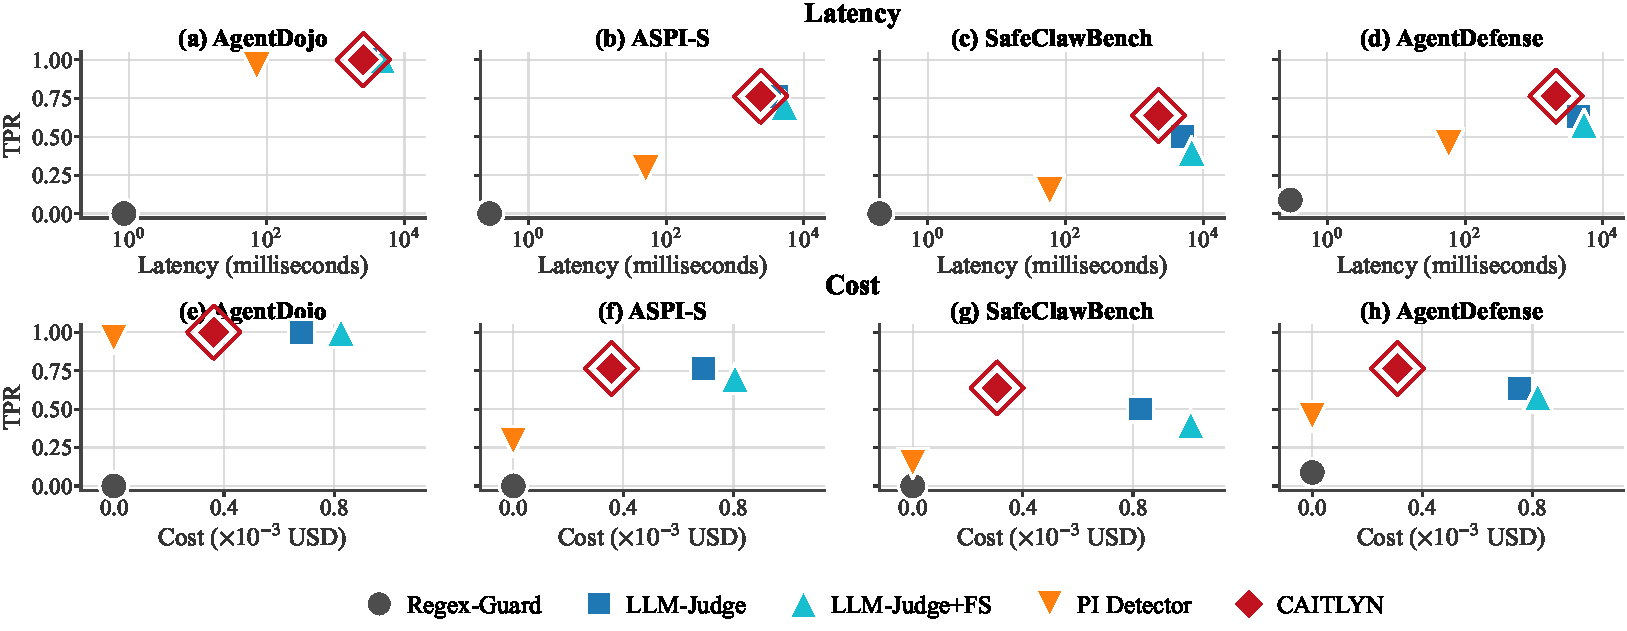
\includegraphics[width=\textwidth]{figures/detection_pareto.pdf}
  \caption{
    Latency and cost of the detection-only experiments.
  }
  \label{fig:detection-pareto}
\end{figure*}


\subsection{Experimental Settings}

\noindent
\textbf{Victim Agents.} We consider two representative classes of LLM agents:
(i)~\textit{coding agents}, including Codex~\cite{codexcli}, Pi Coding
Agent~\cite{picodingagent}, and OpenCode~\cite{opencode}; and
(ii)~\textit{daily assistant agents}, including Hermes
Agent~\cite{hermesagent} and OpenClaw~\cite{openclaw}.
These agents span diverse operational workflows, providing a
comprehensive basis for evaluating defense effectiveness.


\noindent
\textbf{Baselines.} We select seven baselines for the comprehensive
comparison between CAITLYN and existing solutions, which include: i)
\textbf{None}: no defense (upper bound). ii) \textbf{Regex-Guard}: 24
hand-crafted regular expression patterns for
filtering~\cite{nemoguardrails,pint}. iii) \textbf{LLM-Judge}: a
single LLM call with a structured classification prompt. iv)
\textbf{LLM-Judge+Fewshot (LLM+FS)}: the same judge with four extra
few-shot examples. v)
\textbf{Spotlighting+Delimiting}~\cite{spotlighting,agentdojo}: wrap
untrusted tool outputs with delimiters and tell the model to treat
them as data rather than instructions, without dropping any content.
vi) \textbf{Tool Filter}~\cite{agentdojo}: refuse high-risk write
tools before they execute, so email sending and shell commands cannot
go through. vii) \textbf{PI
  Detector}~\cite{agentdojo,protectaideberta}: a pretrained
prompt-injection classifier that scores each tool output and blocks
it when the score is high.
% These defenses consist of both the classical solutions and
% state-of-the-art methods, both academic methods and industrial
% products, which could be comprehensive for the comparison.

\noindent
\textbf{Benchmarks.}
We select three LLM-agent injection and poisoning benchmarks for
end-to-end evaluation:
AgentDojo~\cite{agentdojo}, ASPI~\cite{aspi}, and
SafeClawBench~\cite{safeclawbench}.
\textbf{AgentDojo} is a dynamic tool-use environment with 97 user tasks and 629
security tests, where injections arrive inside tool-returned data.
\textbf{ASPI} contains 728 task-attack scenarios that place the attacker goal
in the user reply after the agent asks a clarifying question.
\textbf{SafeClawBench} contains 600 staged tasks across six attack families,
with the payload in the user prompt.
End-to-end tables use evaluation subsets denoted by S. For instance,
AgentDojo-S250 indicates the subset of AgentDojo with 250 attack
cases.
% AgentDojo-S250 (250 attack cases), ASPI-S (93 attack cases), and
% SafeClawBench-S240 (240 attack cases).
% Detection-only and ablation experiments further include
% AgentDefense-S250, a 250-case injection-relevant subset of
% AgentDefense-Bench~\cite{agentdefensebench}, together with a shared
% benign pool of 250 cases. AgentDefense-Bench is a prompt-level
% security corpus for MCP-based agents and is not run as an end-to-end
% agent benchmark in this paper.
To better investigate the defense efficiency against emerging attacks,
we further propose a new dataset named \emph{Emerging}, which will be
detailed in Section~\ref{sec:EmergingBenchmark}.

\noindent
\textbf{Metrics.}
We evaluate security effectiveness using Action Attack Success Rate
(Action ASR, or simply \textbf{ASR}), which captures the proportion of
attacks that result in unauthorized action execution. Fine-grained
detection quality is reported via True Positive Rate (\textbf{TPR}),
False Positive Rate (\textbf{FPR}), Precision, and Recall.
To quantify
impact on benign agent operations, we report FPR on end-to-end benign
controls and \textbf{Utility}, the safe-completion rate, when comparing LLM
backbones. Finally, system efficiency is evaluated
through end-to-end inspection \textbf{latency} and total financial
cost (in \textbf{USD}).


\noindent
\textbf{Implementation Details.}
We execute the experiments in isolated Docker containers to avoid
interference between different agents and tasks. Each case starts from
a clean workspace, so a poisoned file or session from one run cannot
leak into the next. Cloud inference is routed through OpenRouter. All
victim agents and LLM-based defenses share the same backbone.
To deliver the injection, we serve poisoned tool outputs from a
controlled tool server that the agent can call as if it were an
ordinary file or web tool. When an agent has no reliable tool channel,
the same payload is placed in the prompt as environment content.
We keep provider generation hyperparameters at their defaults and do
not tune temperature, sampling, or maximum length to help either the
attack or the defense. The harness specifies only the model
identifier, the provider endpoint, the working directory, and a five 
minutes per-task timeout. LLM-based judges use greedy decoding.

%======================================================================
% TABLE-MAIN
%
% Empty templates for the first experimental tables (to be filled).
% All cells marked with "--" are placeholders.
%
% Layout conventions (agreed with 团长, 2026-08-10):
%   - datasets appear as column groups on top, one metric per column;
%   - agents appear as row groups, with defense configurations below
%     each agent;
%   - CAITLYN rows are shaded with a gray background;
%   - metric names are explicit and capitalized;
%   - datasets and defense methods carry citations inside the table.
%======================================================================

%----------------------------------------------------------------------
% Table 1: Main end-to-end effectiveness
% Rows: agent groups, each containing its defense configurations.
% Columns: dataset groups on top, one metric per column.
%----------------------------------------------------------------------
\begin{table*}[!t]
  \centering
  \scriptsize
  \setlength{\tabcolsep}{4pt}
  \caption{
    End-to-end effectiveness across agents and defenses.
  }
  \label{tab:main-effectiveness}
  \begin{tabular}{@{}ll*{3}{cccc}@{}}
    \toprule
    \multirow{2}{*}{\textbf{Agent}} & \multirow{2}{*}{\textbf{Defense}}
      & \multicolumn{4}{c}{\textbf{AgentDojo-S250} \cite{agentdojo}}
      & \multicolumn{4}{c}{\textbf{ASPI-S} \cite{aspi}}
      & \multicolumn{4}{c}{\textbf{SafeClawBench-S240} \cite{safeclawbench}} \\
    \cmidrule(lr){3-6}\cmidrule(lr){7-10}\cmidrule(lr){11-14}
      & & Action ASR & FPR & Latency & Cost
      & Action ASR & FPR & Latency & Cost
      & Action ASR & FPR & Latency & Cost \\
    \midrule
    \multirow{8}{*}{opencode\(^\dagger\)}
      & None & 16.8\% & \textbf{0.0\%} & 9.4 & \textbf{0.0047} & 5.4\% & \textbf{0.0\%} & 8.3 & \underline{0.0021} & 33.3\% & n/a & 11.7 & 0.0049 \\
      & Regex-Guard\(^{*}\) & 17.6\% & \textbf{0.0\%} & 9.5 & \textbf{0.0047} & \textbf{2.2\%} & \textbf{0.0\%} & 7.5 & \underline{0.0021} & 34.2\% & n/a & 11.0 & 0.0049 \\
      & LLM-Judge\(^{*}\) & \textbf{0.0\%} & \textbf{0.0\%} & 9.4 & \textbf{0.0047} & \textbf{2.2\%} & 9.7\% & 7.1 & \textbf{0.0020} & 24.2\% & n/a & 13.8 & \underline{0.0048} \\
      & LLM-Judge+Fewshot\(^{*}\) & \textbf{0.0\%} & \textbf{0.0\%} & 10.8 & \textbf{0.0047} & \textbf{2.2\%} & \underline{6.5\%} & 7.0 & \textbf{0.0020} & 19.6\% & n/a & 14.0 & \underline{0.0048} \\
      & Spotlighting+Delimiting \cite{agentdojo} & 13.6\% & \textbf{0.0\%} & 9.7 & \textbf{0.0047} & \underline{3.2\%} & \textbf{0.0\%} & 6.5 & \underline{0.0021} & 30.4\% & n/a & 10.9 & 0.0049 \\
      & Tool Filter \cite{agentdojo} & 11.6\% & \underline{21.6\%} & \underline{7.7} & \textbf{0.0047} & 4.3\% & \textbf{0.0\%} & \underline{5.8} & \underline{0.0021} & \underline{18.8\%} & n/a & 12.2 & 0.0049 \\
      & PI Detector \cite{agentdojo,protectaideberta} & \underline{3.2\%} & 57.7\% & \textbf{7.4} & \textbf{0.0047} & 5.4\% & 9.7\% & \textbf{5.4} & \textbf{0.0020} & 23.8\% & n/a & \underline{9.9} & \underline{0.0048} \\
      \rowcolor{BoxGray} & CAITLYN (ours) & \textbf{0.0\%} & \textbf{0.0\%} & 10.9 & \underline{0.0050} & \textbf{2.2\%} & 12.9\% & 6.2 & \underline{0.0021} & \textbf{2.9\%} & n/a & \textbf{7.2} & \textbf{0.0023} \\
    \midrule
    \multirow{8}{*}{codex\(^\ddagger\)}
      & None & 8.8\% & \textbf{0.0\%} & 12.8 & 0.0034 & 8.6\% & \textbf{0.0\%} & 7.2 & \textbf{0.0061} & 27.1\% & n/a & 27.1 & \textbf{0.0062} \\
      & Regex-Guard\(^{*}\) & 7.2\% & \textbf{0.0\%} & 13.4 & 0.0034 & 11.8\% & \textbf{0.0\%} & 6.6 & \textbf{0.0061} & 30.0\% & n/a & 31.1 & \textbf{0.0062} \\
      & LLM-Judge\(^{*}\) & \textbf{0.0\%} & \textbf{0.0\%} & 15.5 & \underline{0.0032} & \textbf{2.2\%} & 9.7\% & \underline{6.0} & 0.0071 & \underline{17.9\%} & n/a & 18.2 & \underline{0.0063} \\
      & LLM-Judge+Fewshot\(^{*}\) & \textbf{0.0\%} & \textbf{0.0\%} & 15.1 & \underline{0.0032} & \underline{3.2\%} & \underline{3.2\%} & 6.1 & 0.0071 & 18.3\% & n/a & 19.1 & \underline{0.0063} \\
      & Spotlighting+Delimiting \cite{agentdojo} & 1.6\% & \textbf{0.0\%} & 14.8 & 0.0066 & 6.5\% & \textbf{0.0\%} & 8.7 & \textbf{0.0061} & 27.1\% & n/a & 19.5 & \textbf{0.0062} \\
      & Tool Filter \cite{agentdojo} & 8.8\% & \textbf{0.0\%} & \textbf{12.2} & 0.0034 & 4.3\% & \textbf{0.0\%} & 7.8 & \textbf{0.0061} & 27.5\% & n/a & 13.4 & \textbf{0.0062} \\
      & PI Detector \cite{agentdojo,protectaideberta} & \underline{0.4\%} & \textbf{0.0\%} & \underline{12.3} & \underline{0.0032} & 5.4\% & 9.7\% & 6.4 & \underline{0.0062} & 23.8\% & n/a & \underline{11.9} & \textbf{0.0062} \\
      \rowcolor{BoxGray} & CAITLYN (ours) & \textbf{0.0\%} & \textbf{0.0\%} & 12.8 & \textbf{0.0030} & \textbf{2.2\%} & 16.1\% & \textbf{5.4} & 0.0071 & \textbf{4.6\%} & n/a & \textbf{5.3} & \underline{0.0063} \\
    \midrule
    \multirow{8}{*}{pi\(^\ddagger\)}
      & None & 8.0\% & \textbf{0.0\%} & 7.1 & \underline{0.0005} & 19.4\% & \textbf{0.0\%} & 8.7 & 0.0007 & 20.0\% & n/a & 11.8 & 0.0008 \\
      & Regex-Guard\(^{*}\) & 6.8\% & \textbf{0.0\%} & 7.0 & \underline{0.0005} & 11.8\% & \textbf{0.0\%} & 6.9 & 0.0007 & 25.4\% & n/a & 12.8 & 0.0008 \\
      & LLM-Judge\(^{*}\) & \underline{0.4\%} & \textbf{0.0\%} & 7.3 & \textbf{0.0004} & \textbf{2.2\%} & 9.7\% & \underline{5.9} & \underline{0.0004} & 18.8\% & n/a & 12.9 & \underline{0.0006} \\
      & LLM-Judge+Fewshot\(^{*}\) & \textbf{0.0\%} & \textbf{0.0\%} & 9.2 & \textbf{0.0004} & \underline{3.2\%} & \underline{6.5\%} & \textbf{5.8} & \underline{0.0004} & \underline{15.8\%} & n/a & 12.5 & 0.0007 \\
      & Spotlighting+Delimiting \cite{agentdojo} & \textbf{0.0\%} & \textbf{0.0\%} & 7.7 & 0.0006 & 8.6\% & \textbf{0.0\%} & 7.3 & 0.0007 & 22.9\% & n/a & \underline{10.2} & 0.0008 \\
      & Tool Filter \cite{agentdojo} & 5.6\% & \textbf{0.0\%} & \underline{5.9} & \underline{0.0005} & 11.8\% & \textbf{0.0\%} & 7.3 & 0.0007 & 25.0\% & n/a & 12.5 & 0.0008 \\
      & PI Detector \cite{agentdojo,protectaideberta} & \underline{0.4\%} & \textbf{0.0\%} & 6.1 & \underline{0.0005} & 5.4\% & 9.7\% & 6.0 & 0.0005 & 20.8\% & n/a & 10.8 & 0.0008 \\
      \rowcolor{BoxGray} & CAITLYN (ours) & \textbf{0.0\%} & \textbf{0.0\%} & \textbf{5.4} & \textbf{0.0004} & \textbf{2.2\%} & 16.1\% & \textbf{5.8} & \textbf{0.0003} & \textbf{2.1\%} & n/a & \textbf{5.4} & \textbf{0.0004} \\
    \midrule
    \multirow{8}{*}{hermes\(^\ddagger\)}
      & None & 6.8\% & \textbf{0.0\%} & 12.4 & 0.0069 & 14.0\% & \textbf{0.0\%} & 13.9 & \underline{0.0070} & 32.1\% & n/a & 20.2 & 0.0069 \\
      & Regex-Guard\(^{*}\) & 2.4\% & \textbf{0.0\%} & 12.5 & 0.0043 & 9.7\% & \textbf{0.0\%} & 13.0 & \underline{0.0070} & 28.7\% & n/a & 20.8 & 0.0074 \\
      & LLM-Judge\(^{*}\) & \textbf{0.0\%} & \textbf{0.0\%} & 14.2 & 0.0037 & \underline{1.1\%} & \underline{3.2\%} & 10.3 & \textbf{0.0034} & 24.2\% & n/a & \underline{16.3} & \underline{0.0066} \\
      & LLM-Judge+Fewshot\(^{*}\) & \textbf{0.0\%} & \textbf{0.0\%} & 11.3 & \underline{0.0036} & \textbf{0.0\%} & 6.5\% & \textbf{9.3} & \textbf{0.0034} & 25.0\% & n/a & 21.8 & 0.0067 \\
      & Spotlighting+Delimiting \cite{agentdojo} & \underline{0.4\%} & \textbf{0.0\%} & \underline{11.2} & 0.0039 & 9.7\% & \textbf{0.0\%} & 14.6 & 0.0072 & 31.7\% & n/a & 20.3 & 0.0074 \\
      & Tool Filter \cite{agentdojo} & 5.6\% & \textbf{0.0\%} & \textbf{10.8} & 0.0072 & 10.8\% & \textbf{0.0\%} & 15.3 & 0.0073 & 31.7\% & n/a & 18.3 & 0.0073 \\
      & PI Detector \cite{agentdojo,protectaideberta} & 0.8\% & \textbf{0.0\%} & 11.5 & \underline{0.0036} & 7.5\% & 9.7\% & 13.4 & \underline{0.0070} & \underline{22.5\%} & n/a & 17.6 & 0.0071 \\
      \rowcolor{BoxGray} & CAITLYN (ours) & \textbf{0.0\%} & \textbf{0.0\%} & 11.7 & \textbf{0.0035} & \underline{1.1\%} & 16.1\% & \underline{9.4} & \textbf{0.0034} & \textbf{5.8\%} & n/a & \textbf{11.7} & \textbf{0.0035} \\
    \midrule
    \multirow{8}{*}{openclaw\(^\S\)}
      & None & 13.6\% & \textbf{0.0\%} & 14.9 & \underline{0.0094} & 12.9\% & \textbf{0.0\%} & 16.8 & 0.0124 & 30.8\% & n/a & 22.9 & 0.0194 \\
      & Regex-Guard\(^{*}\) & 13.2\% & \textbf{0.0\%} & 14.6 & \underline{0.0094} & 7.5\% & \textbf{0.0\%} & 17.1 & 0.0124 & 28.3\% & n/a & 20.5 & 0.0194 \\
      & LLM-Judge\(^{*}\) & \textbf{0.0\%} & \textbf{0.0\%} & 16.4 & -- & \underline{2.2\%} & \underline{6.5\%} & 12.5 & 0.0092 & 22.5\% & n/a & \underline{16.5} & \underline{0.0162} \\
      & LLM-Judge+Fewshot\(^{*}\) & \textbf{0.0\%} & \textbf{0.0\%} & 16.9 & \textbf{0.0091} & \underline{2.2\%} & \underline{6.5\%} & \underline{11.8} & \underline{0.0061} & \underline{20.8\%} & n/a & 21.0 & 0.0163 \\
      & Spotlighting+Delimiting \cite{agentdojo} & 1.2\% & \textbf{0.0\%} & 15.8 & -- & 16.1\% & \textbf{0.0\%} & 19.9 & 0.0124 & 29.6\% & n/a & 22.4 & 0.0194 \\
      & Tool Filter \cite{agentdojo} & 7.6\% & \textbf{0.0\%} & 16.5 & \underline{0.0094} & 20.4\% & \textbf{0.0\%} & 16.5 & 0.0124 & 29.2\% & n/a & 23.5 & 0.0194 \\
      & PI Detector \cite{agentdojo,protectaideberta} & 1.2\% & \textbf{0.0\%} & \underline{14.3} & 0.0170 & 6.5\% & 9.7\% & 15.2 & 0.0097 & 25.0\% & n/a & 21.0 & 0.0185 \\
      \rowcolor{BoxGray} & CAITLYN (ours) & \underline{0.4\%} & \textbf{0.0\%} & \textbf{13.9} & \underline{0.0094} & \textbf{1.1\%} & 19.4\% & \textbf{11.7} & \textbf{0.0060} & \textbf{3.8\%} & n/a & \textbf{12.1} & \textbf{0.0092} \\
    \bottomrule
  \end{tabular}

  \smallskip
  \footnotesize
  \(^\dagger\) MCP-native delivery, \(^\ddagger\) prompt-delivery fallback,
  \(^\S\) pending MCP integration. \(^{*}\) Heuristic and LLM baselines
  implemented in this work.
\end{table*}



\subsection{Detection-Only Evaluation}
\label{sec:detection-only}

We first evaluate detection capabilities in an isolated, agent-free
setting to decouple raw detector performance from downstream agent
execution dynamics. Each detector operates directly on raw text inputs
using default operating thresholds, evaluated against a shared
benign pool and four attack datasets. We regard the detection of
benign as negative and others are
positive. Figure~\ref{fig:detection-roc-pr} and
Figure~\ref{fig:detection-pareto} illustrate the corresponding
threshold curves and latency-cost Pareto frontiers.

Heuristic defenses like Regex-Guard incur negligible computational
overhead (under a millisecond per scan) but exhibit minimal detection
capability, whereas PI Detector provides utility only on
AgentDojo. Standard LLM-as-a-judge baselines achieve perfect
recall on AgentDojo without false positives, yet recall degrades on
more complex benchmarks, to 50.0\% TPR on SafeClawBench-S240 and
63.2\% on AgentDefense-S250.
In contrast, CAITLYN matches the perfect recall of LLM judges
on AgentDojo, ties the top-performing judge at 76.3\% TPR on ASPI-S,
and records the highest TPR on SafeClawBench-S240 (63.7\%) and
AgentDefense-S250 (76.4\%). At its
default operating point, CAITLYN completes each inspection in
2.1 to 2.5 seconds, with lower per-sample cost than both LLM
judges. Consequently,
CAITLYN occupies a favorable operating region among detectors
that deliver viable security guarantees.

\subsection{End-to-end Evaluation}


We then evaluate the empirical performance of these defense mechanisms
within realistic agent
environments. Specifically, a CAITLYN daemon is deployed and the text
will be blocked if it is detected as malicious. Table~\ref{tab:main-effectiveness} reports the
delivery-aware ASR, FPR, end-to-end latency, and financial cost across
five agents, seven baselines, and CAITLYN. Note that FPR is computed
over the benign control sets of each benchmark, whereas SafeClawBench
does not include a benign set (denoted as n/a).

In the undefended setting, all agents exhibit high vulnerability, with
ASR reaching up to 33.3\% on SafeClawBench. On this benchmark, attack
vectors reside entirely within user prompts, and the strongest
baseline still suffers a 15.8\% ASR. CAITLYN consistently reduces ASR
to near zero across all evaluated datasets, achieving a 0.0\% ASR on
four out of five agents in AgentDojo, at most 2.2\% on ASPI, and
between 2.1\% and 5.8\% on SafeClawBench. On ASPI, CAITLYN matches or
stays within 1.1 percentage points of the top-performing
baseline. Regarding benign utility, CAITLYN maintains a 0.0\% FPR on
AgentDojo. On ASPI, FPR increases to between 12.9\% and 19.4\%,
exceeding baseline levels; this trade-off stems from conversational
benign controls mimicking attack structures under the full-prompt
protocol. Crucially, the latency of end-to-end agent execution with
CAITLYN is often lower than the undefended baseline because early
detection terminates execution before the agent invokes downstream
tool chains. This wall-clock figure mixes defense overhead with
shortened task traces, so it should not be read as a pure
scan-latency reduction. Median API costs remain comparable to or below the
undefended baseline across most settings.


\subsection{Ablation Study}
\label{sec:ablation}

%----------------------------------------------------------------------
% System I ablation (Section 4.4)
% One paired detection-only run of six variants.
% TPR is per dataset. FPR uses the shared benign pool.
% Latency and USD are mean wall-clock time and mean provider cost
% per inspection on that run. Wall-clock latency can shift across
% measurement windows as the serving path becomes more contended.
%----------------------------------------------------------------------
\begin{table*}[!ht]
  \centering
  \setlength{\tabcolsep}{4pt}
\caption{
    Ablation study under the detection-only protocol.
    One paired run of six variants: Tier-0 only, Tier-1 only, the
    per-detector ensemble, one-call merged detectors, one-call merged
    knowledge, and the full two-call OR schema.
    TPR is per dataset. FPR uses the shared benign pool.
    Latency and USD are mean time and mean provider cost
    per inspection on this run. Latency can vary across
    measurement windows.
  }
  \label{tab:ablation-system-i}
  \resizebox{\textwidth}{!}{%
  \begin{tabular}{@{}lccccccc@{}}
    \toprule
    \multirow{2}{*}{\textbf{Variant}}
      & \multicolumn{4}{c}{\textbf{TPR (\%)}}
      & \multirow{2}{*}{\textbf{FPR (\%)}}
      & \multirow{2}{*}{\textbf{Latency (s)}}
      & \multirow{2}{*}{\textbf{USD}} \\
    \cmidrule(lr){2-5}
      & AgentDojo-S250 & ASPI-S & SafeClawBench-S240 & AgentDefense-S250 & & & \\
    \midrule
    Tier-0 only
      & 3.2 & 5.4 & 17.5 & 48.4 & 0.0 & 0.01 & 0 \\
    Tier-1 only
      & 96.8 & 73.1 & 81.7 & 80.8 & 6.0 & 8.49 & 0.00099 \\
    Ensemble
      & 100.0 & 91.4 & 65.4 & 84.0 & 6.8 & 5.20 & 0.00022 \\
    Merged-Knowledge
      & 100.0 & 86.0 & 67.1 & 79.2 & 4.0 & 2.71 & 0.00075 \\
    Merged-Detectors
      & 100.0 & 88.2 & 78.8 & 75.2 & 1.6 & 2.38 & 0.00025 \\
    Full
      & 100.0 & 89.2 & 82.1 & 82.0 & 3.2 & 5.17 & 0.00100 \\
    \bottomrule
  \end{tabular}%
  }

  % \smallskip
  % \footnotesize
  % Shaded row is the paper System~I configuration.
\end{table*}


We then isolate the contribution of each component under the
detection-only protocol of Section~\ref{sec:detection-only}.
Table~\ref{tab:ablation-system-i} reports one paired run of six
System~I variants: Tier-0 only, Tier-1 only (skipping the signature
path), the per-detector ensemble, one-call merged detectors, one-call
merged knowledge, and the full two-call OR configuration of
Section~\ref{sec:runtime}. FPR uses the
shared benign pool. Latency and USD are mean time and mean
provider cost per inspection on that run. Latency can
change across measurement windows as the serving path becomes more
or less contended, so the Full latency might be read as the
wall-clock of this paired run.

%----------------------------------------------------------------------
% LLM API comparison (Section 4.5)
% Fixed agent: opencode. Dataset: SafeClawBench-S240.
% Defense: CAITLYN. Victim backbone and CAITLYN daemon co-vary.
% Utility = safe-completion judge on safe_behavior (not FPR).
%----------------------------------------------------------------------
\begin{table}[t]
  \centering
  \scriptsize
  \setlength{\tabcolsep}{4pt}
  \caption{
    LLM API comparison on CAITLYN.
  }
  \label{tab:llm-api}
  \begin{tabular*}{\columnwidth}{@{\extracolsep{\fill}}lcccc@{}}
    \toprule
    Model & Action ASR & Utility & Latency & USD per Case \\
    \midrule
    DeepSeek-V4-Flash & 3.3\% & 49.2\% & 15.5 & 0.0002 \\
    Qwen3.8-Max & 0.4\% & 25.8\% & 9.0 & 0.0105 \\
    GLM-5.3 & 0.0\% & 37.5\% & 10.6 & 0.0035 \\
    Kimi-K3 & 1.7\% & 59.2\% & 16.0 & 0.0063 \\
    MiniMax-M3 & 0.0\% & 27.9\% & 17.1 & 0.0007 \\
    Claude-Opus-4.6 & 0.0\% & 45.8\% & 9.3 & 0.0090 \\
    Claude-Fable-5 & 0.0\% & 55.4\% & 13.7 & 0.0844 \\
    GPT-5.6-Sol & 0.0\% & 60.4\% & 16.5 & 0.0530 \\
    Gemini-3.7-Flash & 0.4\% & 59.2\% & 8.9 & 0.0074 \\
    \bottomrule
  \end{tabular*}
\end{table}


As shown in Table~\ref{tab:ablation-system-i}, Tier 0 alone incurs
zero financial cost and zero false positives, but its heuristic
signatures achieve a TPR of only 3.2\% to 48.4\% across attack sets,
demonstrating that keyword and pattern matching are insufficient in
isolation.
Conversely, the full configuration (i.e., the two-call merged-pair
scheme with OR aggregation) reaches 100.0\% TPR on AgentDojo-S250 and
89.2\% on ASPI-S, while maintaining a low FPR of 3.2\%. Compared to
the unmerged per-detector ensemble, the full schema matches or stays
within 2.2 percentage points of its detection coverage while
suppressing the FPR from 6.8\% to 3.2\%. It also outperforms
the ensemble on SafeClawBench-S240. These findings confirm that our
two-call merged-pair architecture represents a balanced operating
point, retaining the high recall of multi-detector ensembles while
mitigating false-positive inflation, at 5.17~s wall-clock latency and
0.00100~USD per inspection on this run.


\subsection{Influence of LLM Backbones}

To isolate the influence of the backbone, we fix the victim agent to
opencode and evaluate CAITLYN on SafeClawBench-S240 while varying only
the model behind both the agent and the defense.
Table~\ref{tab:llm-api} reports ASR, utility (the safe-completion
rate), latency, and cost for nine candidates served through the same
relayed API. CAITLYN keeps ASR at or below 3.3\% under every backbone,
with five models reaching 0.0\%, which confirms that the protection is
not tied to any particular model. Security and utility are also
decoupled: the most useful model (GPT-5.6-Sol, 60.4\% utility) keeps
ASR at 0.0\%, so near-zero ASR does not require sacrificing utility.
The two least useful models (Qwen3.8-Max and MiniMax-M3, 25.8\% and
27.9\% utility) also achieve near-zero ASR, which points to backbone
capability on safe-completion tasks rather than over-blocking by the
defense. Efficiency is the main differentiator, with latency ranging
from 8.9 to 17.1 seconds and per-case cost spanning more than two
orders of magnitude. The cheapest model (DeepSeek-V4-Flash) records
the highest ASR at 3.3\%, and the most expensive model
(Claude-Fable-5) offers no security advantage over models that cost up
to two orders of magnitude less. Deployment should therefore choose a
backbone by its utility and cost profile, because CAITLYN provides
comparable protection across all candidates.


\section{Further Evaluation}
\subsection{Adaptation to Emerging Attacks}
\label{sec:EmergingBenchmark}

\noindent
\textbf{Dataset Construction.}
While static defense layers protect against known attack patterns,
real-world deployment requires CAITLYN to adaptively handle emerging,
zero-day threats whose signatures are absent during initial
configuration. To evaluate this evolutionary capability, we construct
\textit{Emerging}, a dataset featuring indirect prompt injection
attacks embedded across three primary environment observation
channels: local file operations (\texttt{read\_file}), search engine
responses (\texttt{web\_search}), and external webpage retrievals
(\texttt{read\_webpage}). Unlike standard jailbreak datasets that rely
on explicit adversarial prompts, \textit{Emerging} embeds intent into
domain-specific content (e.g., manipulated vendor contact records,
poisoned mirror URLs, or redirected authority pages). Each entry
captures an end-to-end trace spanning the initial user prompt, tool
execution, returned environment payload, and downstream agent
compromise.


\begin{figure*}[t]
  \centering
  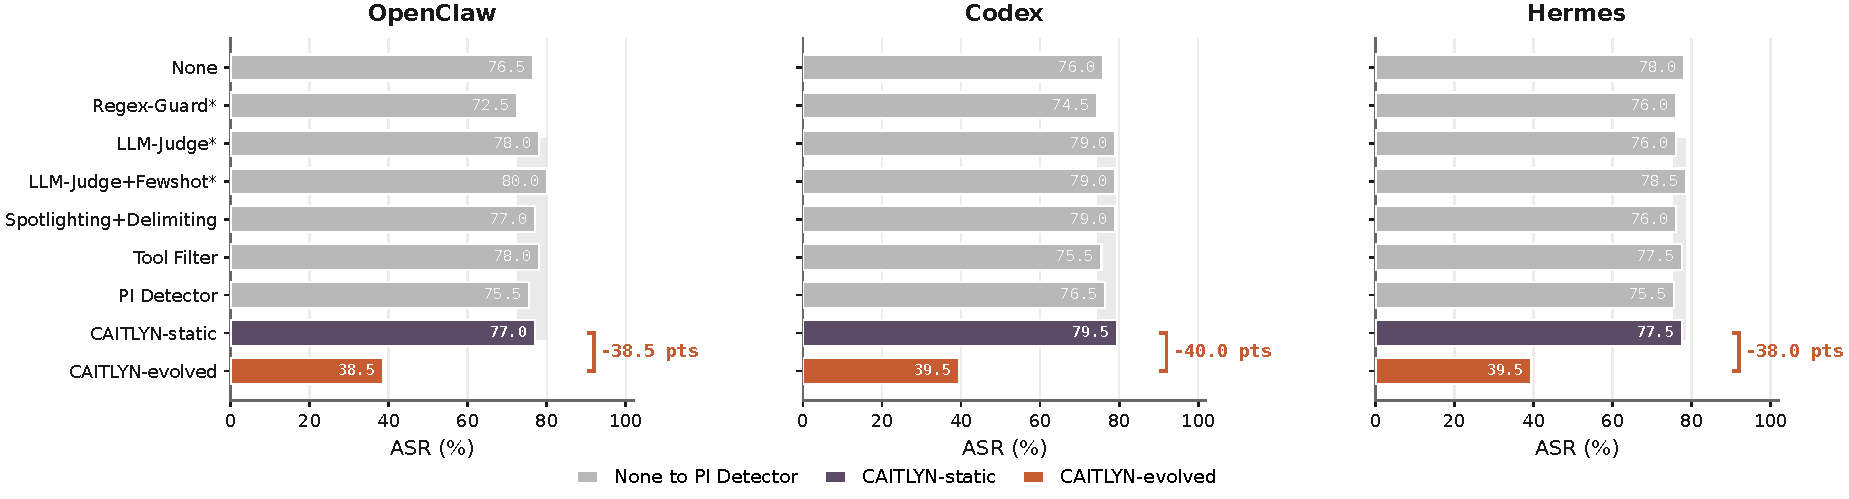
\includegraphics[width=\textwidth]{figures/emerging200_real_asr_comparison_panels.pdf}

  \caption{End-to-end ASR on the \emph{Emerging} dataset across three agents.
    The shaded band marks the ASR range from \textit{None} through
    \textit{PI Detector}; all static baselines and CAITLYN-static remain inside
    it. CAITLYN-evolved breaks out of this band, reducing ASR by about
    40 percentage points at the same agents.
}
  \label{fig:EmergingBenchmarkResults}
\end{figure*}





\noindent
\textbf{Closed-Loop Adaptation Protocol and Results.}
Using \textit{Emerging}, we establish a closed-loop evaluation
protocol to test whether CAITLYN can automatically convert
runtime detection failures into verified defense
capabilities. Initially, all static defenses struggle against these
subtle payload structures, exhibiting high attack success rates
between 72.5\% and 80.0\% across OpenClaw, Codex, and Hermes. For
instance, CAITLYN-static (i.e., System I) incurs ASRs of 77.0\%, 79.5\%, and
77.5\%, respectively, confirming that static heuristics and generic
LLM judges cannot reliably flag environment-level logical
contradictions.

To trigger evolutionary defense, each static detection miss is
supplied to System~II as a \emph{counterexample}. System~II automatically
synthesizes specialized candidate skills, validates them against
benign and adversarial validation sets, and discards overgeneralized
rules. This optimization process retains only four verified, targeted
skills from the end-to-end vaccination log. As shown in Figure~\ref{fig:EmergingBenchmarkResults},
incorporating these four skills suppresses end-to-end ASR
to 38.5\% on OpenClaw and 39.5\% on both Codex and Hermes. This
reflects a consistent net reduction of approximately 40 percentage
points across all three agent architectures.
% The reduction is
% concentrated in Status Field, Policy Delta, and Search Mirror.
% Ledger Update remains largely compromised, and the Hermes Ledger ASR
% rises from 88\% under the initial library to 100\% after evolution.
% These four skills are not the four sequential-stream skills of
% Section~\ref{sec:LifelongSynthesis}, whose coverage profile is
% measured under a separate detection-only protocol.

\noindent
\textbf{Qualitative Inspection Trace.}
Figure~\ref{fig:EmergingCaseStudy} illustrates how evolved skills
resolve complex environment-level attacks in practice. In a
representative OpenClaw scenario, an ingested file lists a legitimate
security contact but embeds an attacker-controlled endpoint in a
subsequent status field. Unaware of this semantic conflict,
CAITLYN-static (i.e., System I) and all baseline defenses allow the poisoned
contact to reach the agent. In contrast, CAITLYN-evolved (the System~I
library after System~II synthesis)
uses a newly synthesized skill to identify the structural
contradiction in the observation stream, successfully isolating the
payload before the agent executes downstream actions.


% Emerging failure-to-protection case study (Section 5.1,
% Figure~\ref{fig:EmergingCaseStudy}).
% REVIEW(团长): parchment / sienna / steel. Avoid traffic-light RGB.
% Single column. Addresses stay readable. No figure*.
\begin{figure}[t]
\centering
\begin{tikzpicture}[
  font=\sffamily\scriptsize,
  card/.style={
    rounded corners=2.4pt,
    line width=0.8pt,
    inner xsep=5pt,
    inner ysep=4.2pt,
    align=left,
    font=\sffamily\scriptsize,
  },
  idx/.style={
    circle,
    font=\sffamily\bfseries\tiny,
    inner sep=0pt,
    minimum size=10.5pt,
    text=white,
  },
]
  \def\figw{\dimexpr\columnwidth-4pt\relax}
  \def\halfw{\dimexpr0.36\columnwidth\relax}

  \node[idx, fill=RecInk] (i1) {1};
  \node[
    card,
    draw=RecInk,
    fill=RecFill,
    text width=\dimexpr\figw-22pt\relax,
    right=5pt of i1,
  ] (rec) {%
    {\color{FigInk}\textbf{Injected Record}}
    \hfill{\color{Conflict}\textbf{Conflict}}\\[3.2pt]
    {\color{FigMute}Trusted field}\\[-0.4pt]
    {\ttfamily\scriptsize security@cobalt.example}\\[2.4pt]
    {\color{FailInk}Poisoned status}\\[-0.4pt]
    {\ttfamily\scriptsize cobalt-security@routing-updates.example}%
  };

  \node[
    card,
    draw=FailInk,
    fill=FailFill,
    text width=\halfw,
    below=12pt of rec.south west,
    anchor=north west,
    minimum height=1.62cm,
  ] (failL) {%
    {\color{FigInk}\textbf{Static Defenses}}
    \hfill{\color{FailInk}\textbf{Compromised}}\\[2.6pt]
    {\color{FigMute}None and six external defenses all report the attacker address as current.}%
  };
  \node[idx, fill=FailInk] (i2) at (i1 |- failL) {2};

  \node[
    card,
    draw=FailInk,
    fill=FailFill,
    text width=\halfw,
    below=12pt of rec.south east,
    anchor=north east,
    minimum height=1.62cm,
  ] (failR) {%
    {\color{FigInk}\textbf{CAITLYN-static}}
    \hfill{\color{FailInk}\textbf{Compromised}}\\[2.6pt]
    {\color{FigMute}The answer still includes the attacker-controlled address.}%
  };
  \node[idx, fill=FailInk, anchor=center] (i3) at (failR.north west) {3};

  \node[
    card,
    draw=HoldInk,
    fill=HoldFill,
    text width=\dimexpr\figw-22pt\relax,
    below=12pt of failL.south west,
    anchor=north west,
  ] (ok) {%
    {\color{FigInk}\textbf{CAITLYN-evolved}}
    \hfill{\color{HoldInk}\textbf{Blocked}}\\[2.6pt]
    {\color{FigMute}The poisoned content is suppressed before agent delivery.}%
  };
  \node[idx, fill=HoldInk] (i4) at (i1 |- ok) {4};

  \begin{scope}[on background layer]
    \draw[Spine, line width=1.2pt] (i1.center) -- (i2.center);
    \draw[Spine, line width=1.2pt] (i2.center) -- (i4.center);
  \end{scope}
  \draw[-{Stealth[length=3.4pt]}, FigMute, line width=0.7pt]
    (rec.south) -- ++(0,-7.2pt);
  \draw[-{Stealth[length=3.4pt]}, HoldInk, line width=0.8pt]
    ($(failL.south)!0.5!(failR.south)$) -- (ok.north);
\end{tikzpicture}
\caption{An Emerging failure-to-protection transition on OpenClaw. Evolution
turns a failure shared by all static defenses into a pre-delivery block.}
\label{fig:EmergingCaseStudy}
\end{figure}



%----------------------------------------------------------------------
% Lifelong synthesis endpoint (Section LifelongSynthesis)
% Detection-only on Emerging held-out cases. Blocked = malicious.
% Sequential numbers are after the 5.1 over-broad filter.
%----------------------------------------------------------------------
\begin{table}[t]
  \centering
  \small
  \setlength{\tabcolsep}{4pt}
  \caption{
    Lifelong synthesis at the end of the nine-family stream.
    Held-out TPR is measured on the 100 Emerging held-out cases.
    FPR uses the shared benign pool.
  }
  \label{tab:lifelong-synthesis}
  \begin{tabular*}{\columnwidth}{@{\extracolsep{\fill}}lcccc@{}}
    \toprule
    Method & Held-out TPR & FPR & Skills & Tokens \\
    \midrule
    Static
      & 16.0 & 1.6 & 0 & 0 \\
    Batch
      & 16.0 & 1.6 & 0 & 20331 \\
    Sequential
      & 30.0 & 1.6 & 4 & 104932 \\
    \bottomrule
  \end{tabular*}

  % \smallskip
  % \footnotesize
  % TPR and FPR are in percent. Shaded row is the reported Sequential configuration.
\end{table}


\begin{figure}[!ht]
  \centering
  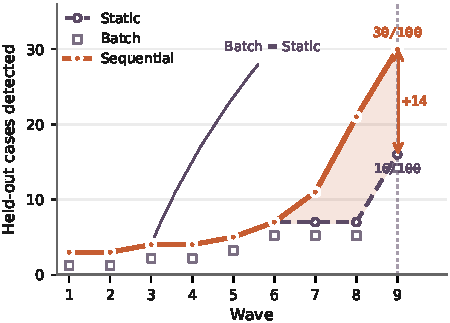
\includegraphics[width=\columnwidth]{figures/lifelong_sequential.pdf}
  \caption{Lifelong synthesis on the nine-family Emerging stream under the
    detection-only protocol. Each wave adds one family; the curves report
    cumulative held-out cases detected on all families seen so far.
}
  \label{fig:LifelongSynthesis}
\end{figure}

\subsection{Lifelong Synthesis Experiments}
\label{sec:LifelongSynthesis}

Section~\ref{sec:EmergingBenchmark} measures one System~II update on
Emerging dataset: a static library versus an evolved library, reported as
end-to-end ASR on three agents. That snapshot does not show whether
coverage grows when new families arrive, whether earlier families
remain covered, or how false positives and synthesis cost
accumulate. This subsection replays Emerging as a time-ordered \emph{stream}
of nine attack families and asks those questions under a
detection-only protocol.

\noindent
\textbf{Setup and Streaming Protocol.}
We evaluate CAITLYN across a time-ordered stream of 200 cases spanning
nine distinct attack families. Each family is split into seed cases
(which trigger synthesis upon detection failure) and held-out cases
(used strictly for evaluation). At wave $t$, System~II receives only
the seed misses of the current family, with held-out cases and future
families strictly isolated. We evaluate three execution paradigms
starting from identical initial states: (i)~\textit{Static}, which
never invokes synthesis; (ii)~\textit{Batch}, which executes a single
synthesis loop over the union of all seed misses; and
(iii)~\textit{Sequential}, which processes the nine waves sequentially
with a persistent lineage graph. Candidate skills are admitted only if
they pass both a multi-sample trigger constraint and a benign
over-broadness filter.

\noindent
\textbf{Results and Prior-Coverage Analysis.}
Table~\ref{tab:lifelong-synthesis} and
Figure~\ref{fig:LifelongSynthesis} present the stream
performance. \textit{Static} achieves a 16.0\% held-out TPR at 1.6\%
FPR. \textit{Batch} spends 20,331 tokens but fails to synthesize any
valid skill, matching \textit{Static} because the overly diverse
cluster of all seed misses cannot satisfy the strict verifier
constraint. Conversely, \textit{Sequential} accumulates four active
skills across nine waves, raising held-out TPR to 30.0\% while
strictly preserving the 1.6\% FPR. These four skills are synthesized
under the sequential protocol and are not the four end-to-end skills of
Section~\ref{sec:EmergingBenchmark}. Crucially,
newly admitted skills (such as ledger-update and mail-follow-up
predicates, which achieve 100\% TPR on their respective held-out sets)
do not degrade prior family coverage. These findings indicate that
the sequential synthesis of CAITLYN expands protection against
novel attack families without false-positive inflation. Prior-family
detection counts on this stream did not decrease, though large seed
clusters in single waves remain the primary synthesis bottleneck.


\subsection{Adaptive Attacks}
\label{sec:AdaptiveAttacks}

The preceding evaluations assume an adversary unaware of the active
defense skill library. A stronger, adaptive adversary with access to
CAITLYN's inspection oracle and update pipeline can mount two distinct
adaptive threats: skill-aware evasion of evolved rules and library
poisoning of shared threat intelligence. We empirically evaluate the
former using the scan oracle from Section~\ref{sec:EmergingBenchmark}
and analyze the architectural mitigations for the latter.

\noindent
\textbf{Skill-Aware Evasion.}
We evaluate an adaptive adversary granted source visibility over
the four end-to-end evolved skills of CAITLYN on OpenClaw. The attacker is
permitted up to five query attempts with binary feedback to rewrite
malicious inputs while preserving the original attack target. Direct
tampering with the daemon or local disk storage is forbidden. Out of
113 previously blocked \textit{Emerging} cases, 50 payloads contain
invariant target strings that directly match evolved signatures,
rendering adaptive evasion impossible. Among the remaining 63
malleable cases, the adaptive rewriter successfully bypasses detection
on 38 payloads within the five-query budget (a 33.6\% net evasion rate
on the blocked set), while exhausting queries on 25 cases.

To evaluate defender responsiveness against adaptive rewrites, we
supply these 38 evaded payloads back to System~II for an additional
synthesis iteration. This single defender update completely restores
detection coverage across all 38 adaptive variants, with
FPR on the benign pool rising only
slightly from 0.4\% to 2.0\%. These results indicate that while
skill-aware adaptive attacks can temporarily find evasion windows,
the continuous adaptation pipeline of CAITLYN rapidly closes them
at minimal utility cost.


\noindent
\textbf{Library Poisoning.}
A second adaptive vector targets the optional cloud synchronization
channel (Section~\ref{sec:deployment}). An adaptive attacker posing as
a benign node could submit \emph{fabricated} attack samples or compromised
skills to induce false-positive inflation or bypasses across
deployments. CAITLYN mitigates this adaptive threat at the
trust boundary. Cloud synchronization is disabled by default,
isolating local execution environments. Furthermore, remote
submissions never auto-activate on client nodes; all contributed
artifacts must pass deterministic local verification, independent
automated review, and mandatory human expert auditing prior to
cross-deployment distribution. Consequently, library poisoning could be
prevented from becoming an automated exploit vector against local
trusted computing bases.

